\documentclass{article}
\usepackage{lineno}
\usepackage[utf8]{inputenc}
\usepackage{geometry}
\usepackage{xcolor}
\usepackage{tikz}
\usepackage{multirow}
\usepackage{natbib}
\usepackage{amssymb}
\usetikzlibrary{shapes,arrows}

\geometry{margin=0.75in}

\title{Evidence for convergent substitutions underlying tetrodotoxin resistance in poison frogs}
\author{Lawrence H. Uricchio, Rebecca D. Tarvin, Juan Carlos Santos, \\ Lauren A. O'Connell (generation of transcriptome data); David C Cannatella (funding); \\ Santiago Ron, Luis Coloma, Marcio Pie, Corinne Richards Zawacki,\\  and Adolfo Amézquita (specimen collection); Harold Zakon (?)}
\date{\today}

\begin{document}
\linenumbers



\maketitle

\begin{abstract}
    Chemical defense is thought to have evolved at least three times in frogs, yet we know relatively little about the evolutionary and genetic mechanisms underlying this widespread ecological strategy. In poison frogs harboring tetrodotoxin, highly conserved sodium channel genes must evolve amino acid substitutions that allow the protein to maintain function in the presence of this lethal toxin. Strong constraints on sodium channel function and a limited repertoire of potentially adaptive mutations could lead to repeated amino acid substitutions in different lineages, or entirely different substitutions may underly the auto-resistance phenotype in each poison frog lineage. Here, we report on an exon-capture sequencing dataset of the alpha subunit of six sodium channel genes across 95 frog species, including 31 species that are known to be poisonous. We apply both selection-based analyses and trait-based analyses to scan for sites that may confer resistance to tetrodotoxin. We report 16 sites that are correlated (after correcting for the phylogeny) with the poison phenotype in genes SCN3A, SCN4A, SCN5A, and SCN8A, suggesting that these alleles may have evolved convergently in different poison frog lineages. We also replicate known resistance sites in SCN4A. Interestingly, none of the newly putatively associated sites overlap known functional domains or resistance sites in poison frogs, and most were not detected by selection scans. We discuss our findings in light of the evolutionary genetics of chemical defense and studies of convergent evolution in general.
    
\end{abstract}


\linespread{1.5}\selectfont
\section*{Introduction}


\begin{enumerate}
    \item general stuff about evolutionary genetics of convergent evolution, what has been tried and what we know (see T. Sackton review)
    \item Poison frogs are an interesting system, some physiological/ecological info 
    \item What we don't know about poison frog system/hy we don't know it
    \item Technical challenges of bait capture, why this is valuable anyway
    \item We generate a new bait-capture dataset to fill some of these gaps. We find ...
\end{enumerate}

\section*{Results}

\subsection*{Assessments of assembly quality}

While computational assembly of DNA sequences from short reads is always a challenge, special considerations arise for bait-capture data. In general, bait-capture is most useful for genes that are sufficiently conserved that a set of high-affinity probes binding the DNA-sequences of interest can be constructed.  In essence this reduces the search space for the assembler by removing sequences that are unlikely to be relevant, but it also discards most intronic sequences, meaning that it is not expected that large contigs can be built. It also means that paralogs of the sequence of interest may be bound by the probes and/or pass BLAST thresholds such that they are incorrectly included in sequence assembly.

In assessing our bait-capture assemblies, we sought to find an appropriate balance between completeness and the inclusion of potential false-positive sequences in our alignments.  Due to the high level of conservation between all pairs of genes included in our analysis (SCN1A, SCN2A, SCN3A, SCN4A, SCN5A, and SCN8A), we were especially concerned about the possible inclusion of chimeric sequences composed of multiple different sodium channels. In general, we do not have a gold standard against which to compare our inferred sequences, so we relied on a series of heuristics to guide our assessments (see Methods). A schematic of our pipeline is displayed in Figure 1.

We tested a wide range of input parameters to \texttt{HybPiper} and two different sets of reference sequences (see Methods). We found that bait sequences composed of a combination of \textit{Oophaga} and \textit{Xenopus} references had better performance than \textit{Xenopus} alone (see Figures S1-S2), and that a small but crucial change to way that \texttt{HybPiper}
distributes reads to gene models resulted in the best overall performance (Figures S3-S4). In general we observe that a more stringent threshold on percent identity between the bait sequence and the reads results in less complete assemblies, and can also result in higher (Fig. S1) or lower (Fig. S2) quality assemblies depending on other choices. When we made a small change to \texttt{HybPiper}'s read distribution function (see Methods) it largely removed the dependence on the threshold parameter. We used these parameter explorations in \texttt{HybPiper} to pick a set of parameters that provided the best balance between completeness of the gene models, settling on \texttt{--thresh 68} and a hybrid bait sequences composed of \textit{Xenopus} and \textit{Oophaga}. \textit{Oophaga} sequences would have been preferred in general since it is a closer relative of the species in our study, but the available gene models are incomplete so we used the \textit{Xenopus} sequences for incomplete regions. 

Lastly, we visually scanned the MSA of each assembled gene for problematic regions and found some regions with 1-2 species that had large insertions not shared with any other species, or short (~10-20) amino acid sequences that were shared between two or three species in different clades but no other species. 

Given the risk of chimeric sequences in  bait capture data, we sought to remove as many of these regions as possible using the software tool \texttt{trimAl} and a final round of manual curation. It is possible that we may have removed some high-quality columns through this trimming, but we were far more concerned with the possibility of false positives. Indeed, none of the SCN2A sequences survived our quality thresholds in \texttt{trimAl}, so we do not report these sequences in our analyses. We suggest that our gene-level selection inferences be taken with caution for this reason. All sequences that we assembled (including SCN2A) and processed are available at \texttt{https://github.com/uricchio/sodiumChannelEvo}, along with \texttt{Snakemake} \citep{koster2012snakemake} pipelines for remaking the data for our figures.

\subsection*{Selection inference}

We used \texttt{BUSTED} and \texttt{MEME} to search for evidence of selection acting across genes and episodically at individual sites, respectively \citep{murrell2015gene,murrell2012detecting}. For our gene level analyses, we subdivided the phylogeny into branches subtended by toxic (foreground) and non-toxic/unknown (background) lineages. We estimated rates of diversification on each of these sets of branches. Notes that since we do not have complete information about toxicity, the background lineages may include some toxic species. Our analysis with \texttt{BUSTED} revealed a higher rate of diversification in SCN4A amongst toxic than non-toxic species (Fig. 2A), which is consistent with adaptive changes in sodium channels to accommodate tetrodotoxin. SCN4A is the only one of the sodium channel genes to be expressed in muscle tissue \cite{gendreau2021gene}, and may be the most exposed to tetrodotoxin in poison frogs. However, \texttt{BUSTED} did not infer substantial differences in the rate of diversifying selection between the foreground and background of any of the genes (Figure 2B).

We were concerned with the possibility that the inclusion of a small number of misaligned sequences could badly distort the findings of \texttt{BUSTED} and \texttt{MEME}. Indeed, \texttt{MEME} identified $\approx 100$ sites as under selection in each gene, and visual inspection of these sites in our alignments suggested that many occurred at the edges of gaps or other possible alignment/assembly errors. We therefore repeated the \citep{BUSTED} analysis using a more conservative trimming strategy in \texttt{trimAl} that removed many more columns from each of the alignments (option \texttt{-st 0.004} rather than {-st 0.001}). We plot the results of this analysis in Figure S6. There was a modest increase in diversification rate $\omega$ for SCN4A, but the difference between background and foreground was very similar. A larger difference between background and foreground was also observed for SCN8A. The other genes had overall similar patterns between the two analyses. We do not report individual branch-site selection statistics from \texttt{MEME} herein because we cannot rule out the possibility of mis-alignment or incorrect assembly at many of the detected sites. However, we do report \texttt{MEME} statistics for the subset of sites that were identified through correlation with toxicity, as this analysis should not be susceptible to the same type of alignment issues.

\subsection*{Correlations with toxicity}

Since toxicity has evolved multiple times in poison frogs, we speculated that alleles conferring resistance to toxicity might have evolved multiple times in different lineages. Indeed, previous work has identified some such sites in SCN4A \citep{tarvin2016convergent,tarvin2017interacting}. We scanned for correlations between amino acid state and toxicity in each column, correcting for the tree structure using PGLS (see Methods). We found 16 sites that survived a $p<0.05$ threshold (Table 1). Note that this is a loose threshold for significance and we do not expect all of these sites to be true positives. However, four of the sites would have passed a much more stringent $p < 1e-4$ threshold.

Figures 3-5 show the correlated sites (along with the phylogeny) for genes SCN4A (Fig.~3), SCN5A (Fig.~4), and SCN5A (Fig.~5). Interestingly, none of the sites intersected eaxctly with known functional domains (such as the p-loop) or known toxicity sites from other species. Known resistance sites (including convergently evolved alleles, such as A445D (Fig.~6; \cite{tarvin2016convergent}). The two most correlated sites both occur in SCN4A (fourth and fifth columns of the MSA in Fig.~3)). Most of these sites would not have been detected with a selection scan, although a few had elevated selection signals (Table 1). 

\section*{Discussion}

\section*{Materials \& Methods}

\subsection*{Sample collection}

{\color{red} Need some info here}.

\subsection*{Sequencing \& sample QC}

Samples were sequenced on an Illumina {\color{red} Hi-Seq? Describe sequencing technology and read quality/depth?}. After obtaining sequence data, we trimmed adaptor sequences and low quality bases from our Illumina short reads using \texttt{TrimGalore} version \texttt{0.6.4\_dev} (\texttt{https://github.com/FelixKrueger/TrimGalore}) using the command \texttt{trim\_galore --paired --phred33 --length 36 -q 20 --stringency 1 --illumina -e 0.1}.

\subsection*{Generating assemblies}
We used \texttt{HybPiper} \cite{johnson2016hybpiper} to generate assemblies of the alpha subunit of six sodium channel genes: SCN1A, SCN2A, SCN3A, SCN4A, SCN5A, SCN8A.  \texttt{HybPiper} combines several other computational tools (including \texttt{BLAST} \cite{altschul1990basic}, \texttt{SPADES} \cite{bankevich2012spades}, and \texttt{exonerate} \cite{slater2005automated}) into a single pipeline that assembles conserved genes from bait-capture sequence data. Details of the computational procedure employed by \texttt{HybPiper} can be found in Johnson \textit{et al} \cite{johnson2016hybpiper}.  Briefly, short reads are first \texttt{BLAST}-ed against a set of bait sequences, which correspond to reference amino acid sequences for the genes of interest from a closely related species. Sequenced reads that obtain an e-value below a user-defined threshold (10e-10 here) against at least one bait sequence are retained for further analysis.  The retained sequences are then provided as input into a short-read assembler (\texttt{SPADES}), which makes reference-guided assemblies using known orthologs of the bait genes as a reference.  Lastly, intron/exon boundaries are inferred by \texttt{exonerate}, and full-length amino acid and nucleic acid sequences are determined for each gene of interest.

Only a limited set of reference sequences are available for sodium channel genes in frogs.  High-quality complete sequences available for \textit{Xenopus tropicalis} and \textit{Xenopus laevis}, and partial sequences from \textit{Oophaga pumilio} and \textit{Rhinella marina}.  Since \textit{Xenopus} is a relatively distant relative of the frogs included in this study, we used \textit{Oophaga pumilio} sequences when possible as bait sequences. Some exons were absent (including the first exon in some cases).  We aligned \textit{Xenopus} and \textit{Oophaga} sequences together for each target gene, and used a custom script (available at \texttt{https://github.com/uricchio/sodiumChannelEvo}) to merge the sequences together, retaining the \textit{Oophaga} sequences when available. These \textit{Xenopus/Oophaga} hybrid sequences were then used as baits in \texttt{HybPiper}, and compared to reference sequences that used only \textit{Xenopus}.

\subsection*{Building gene trees}
We used \texttt{raxml-ng v1.1.0} to build gene trees from our assembled NAV gene sequences \cite{kozlov2019raxml}. We created alignments of the protein coding sequences assembled by \texttt{HybPiper} containing all 6 sodium channel genes for all 95 species using \texttt{mafft} \cite{katoh2005mafft}.  We built the gene trees from the DNA sequences using the command \texttt{raxml-ng --model GTR+G}. 

\subsection*{Assessing our assemblies}
 
Each of step of the \texttt{HybPiper} pipeline (\texttt{BLAST} \citep{altschul1990basic}, \texttt{SPADES} \citep{bankevich2012spades}, and \texttt{exonerate} \citep{slater2005automated}) includes a suite of user-defined options that can affect the quality and completeness of the assemblies. We investigated a range of parameter settings that we hypothesized might affect the performance of the assembler, including the e-value threshold in BLAST, the kmer length in SPADES, the depth multiplier in Exonerarte, and the sequence identity threshold in Exonerate. While each parameter has some effect on the assembled sequences, we focus primarily on the sequence identity threshold here because it had by far the largest effect on the completeness of the sequences (\textit{i.e.}, the length in base pairs of the assembled sequences) and the quality of the gene tress (see Figs. S1-S5 and below).

Assessing the quality of the gene trees is challenging because we do not have a gold standard, and because incomplete lineage sorting, hybridization and other evolutionary processes can complicate the interpretation of gene trees relative to the species tree.  However, it is well known that all six sodium channel genes evolved in the ancestor to all vertebrates, meaning that a well-resolved gene tree should at the very least separate SCN1A, SCN2A, SCN3A, SCN4A, SCN5A, and SCN8A into monophyletic clades.

We assessed the resolution of inferred each gene tree by measuring the number of deep coalescence events that would be required in order for each gene to form its own reciprocally monophyletic clade.  In other words, if zero deep coalescence events are required, then each gene forms its own reciprocally monophyletic clade.  As $X$ increases, the gene trees are increasingly poorly resolved. We used the Python library \texttt{dendropy} to perform this calculation \cite{sukumaran2010dendropy}.

\subsection*{Trimming of poorly aligned columns and sequences}

Despite our best efforts to find parameters that would allow us to build high quality assemblies, visual inspection of the final builds still revealed some sections that included gaps and some sequences with several ($>10$) diverged characters in a row, suggesting assembly errors. While trimming of sequences can have undesirable effects, such as lowering power to detect selection or removing phylogenetically informative characters, we were most concerned about the possibility of false positives given the clear potential for assembly and alignment errors in our bioinformatic pipeline. We therefore decided to further trim bad columns and low performing sequences from our alignments for the purpose of selection analyses. We used \texttt{trimAl} for this processing step \citep{capella2009trimal}. We used the options \texttt{ -resoverlap 0.81 -seqoverlap 80} to trim poorly aligned sequences and subsequently \texttt{-gt 0.6 -st 0.001 -cons 70} to trim poorly aligned columns. We applied a second, more conservative filter on columns  \texttt{-gt 0.6 -st 0.004 -cons 70} in a second round of selection analyses in an attempt to remove some columns that resulted in likely false-positive selection signals (see Results).

Lastly, in the analyses reported in the main text, we manually trimmed some additional columns from sequences that were obviously problematic. These included pairs of sequences that were not closely related but shared 8 or more amino acid characters in common, while most other species had the same highly conserved set of residues in these columns. These sequences are much more likely to represent assembly or alignment errors. 

It is possible that some trimming steps removed legitimate columns or sequences from our assemblies. Therefore, we urge caution in interpreting gene-wide selection inferences we made in this paper, and we note that comparisons across genes are not well founded since each gene has a different set of columns and species removed from the analysis. However, we note that inferences of correlations between amino acid characters and toxicity should not be affected by this issue.   

\subsection*{Testing for selection}

We used the suite of software tools in \texttt{HyPhy} \citep{pond2005hyphy} to test for selection. We used \texttt{BUSTED} \cite{murrell2015gene} to test for selection at the level of entire genes, and \texttt{MEME} \citep{murrell2012detecting} to test for branch-site-specific selection. These methods take a tree and a DNA sequence alignment and fit evolutionary rate models to the data. We used the gene tree for each specific gene in these analyses. \texttt{BUSTED} tests for evidence of selection on a group of foreground lineages, and compares the rate of diversification on the foreground lineages to the complementary set of lineages on the tree (\textit{i.e.}, the background). We specifically sought to infer rates of diversification on branches subtended by toxic species or clades, as compared to species that are not toxic. \texttt{BUSTED} infers 3 rate classes (each of which corresponds to a specific value of $\omega=\frac{dN}{dS}$) and provides estimates of the proportion of sites in each class. Gene trees with the foreground and background lineages denoted are included at \texttt{https://github.com/uricchio/sodiumChannelPaper/Figures/Figure2/plot\_data/}.

\texttt{MEME} tests for evidence of selection at particular sites/branches in the alignment. We hoped to use this method to detect candidate sites for repeated selection across genes or lineages, and sites that might confer toxin resistance.

\subsection*{Testing for correlations with toxicity}

Because toxicity has evolved multiple times on the frog phylogeny, it may be possible to detect substitutions that have evolved convergently in multiple lineages of poison frogs by calculating the correlation between the amino acid state (coded 0/1) and toxicity (coded 0/1). We calculated correlations between sites and toxicity with a custom \texttt{Python} script. Those with correlations exceeding 0.4 were then assessed with an \texttt{R} script that accounted for the phylogenetic structure. For this analysis we used \texttt{ape} and \texttt{phytools} to perform phylogenetic least squares (PGLS) \citep{paradis2004ape,revell2012phytools}. We used the method of Martins and Hansen to account for the phylogeny \citep{martins1997phylogenies}. 
To make our figures, we used \texttt{ggtree} and \texttt{ggmsa} to display trees and alignments, respectively \cite{yu2017ggtree,zhou2022ggmsa}. 


\clearpage
\linespread{1}\selectfont
\section*{Figures \& Tables}

\begin{figure}[h!]
    \centering
    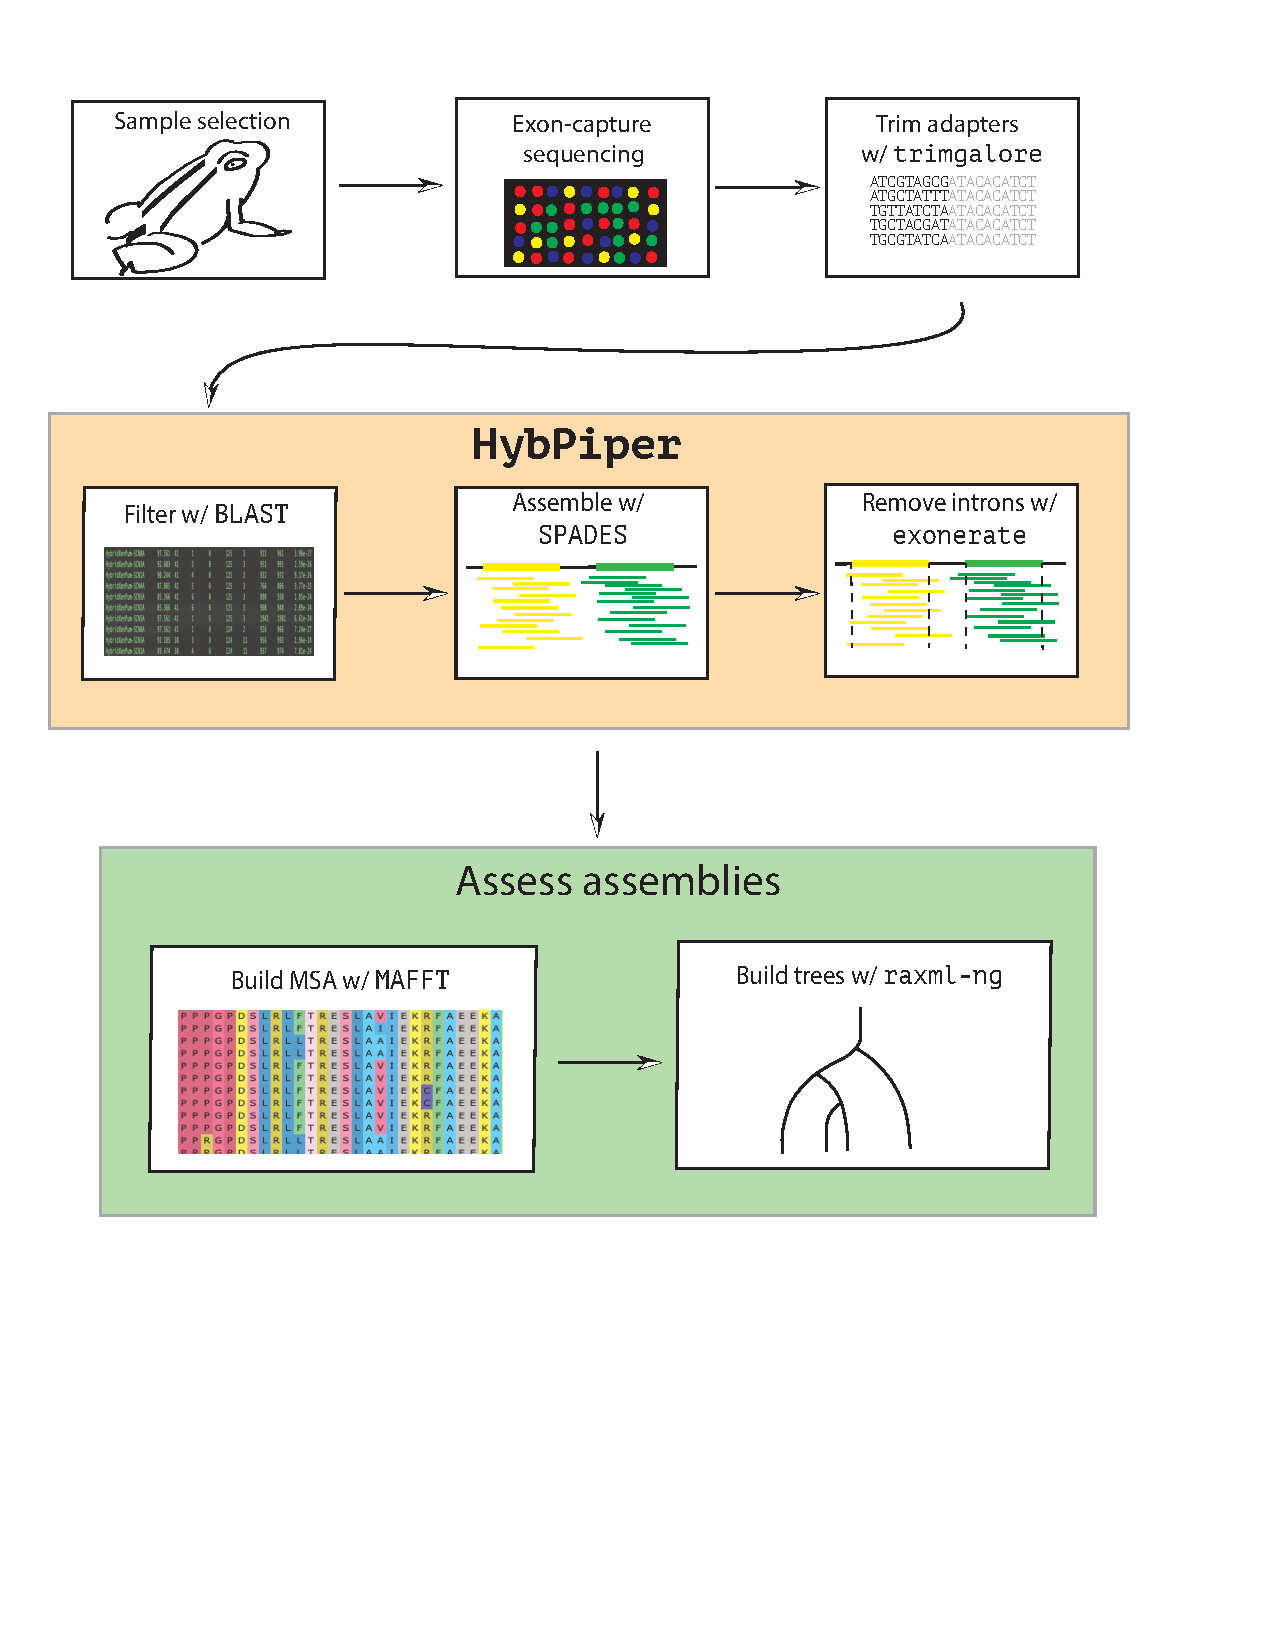
\includegraphics[scale=0.9]{figures/flow_chart.pdf}
    \caption{A flow chart of our assembly pipeline. Bait sequences were used to pull down sodium channels from 97 frog species. We preprocessed these sequences with \texttt{trimgalore} and then used \texttt{HybPiper} to perform reference guided assembly. We assessed assembly quality by building MSAs and gene trees, and comparing the topologies of the gene trees to the expectation of reciprocal monophyly within each sodium channel gene.}
    \label{fig:my_label}
\end{figure}
\clearpage

\begin{figure}[h!]
    \centering
    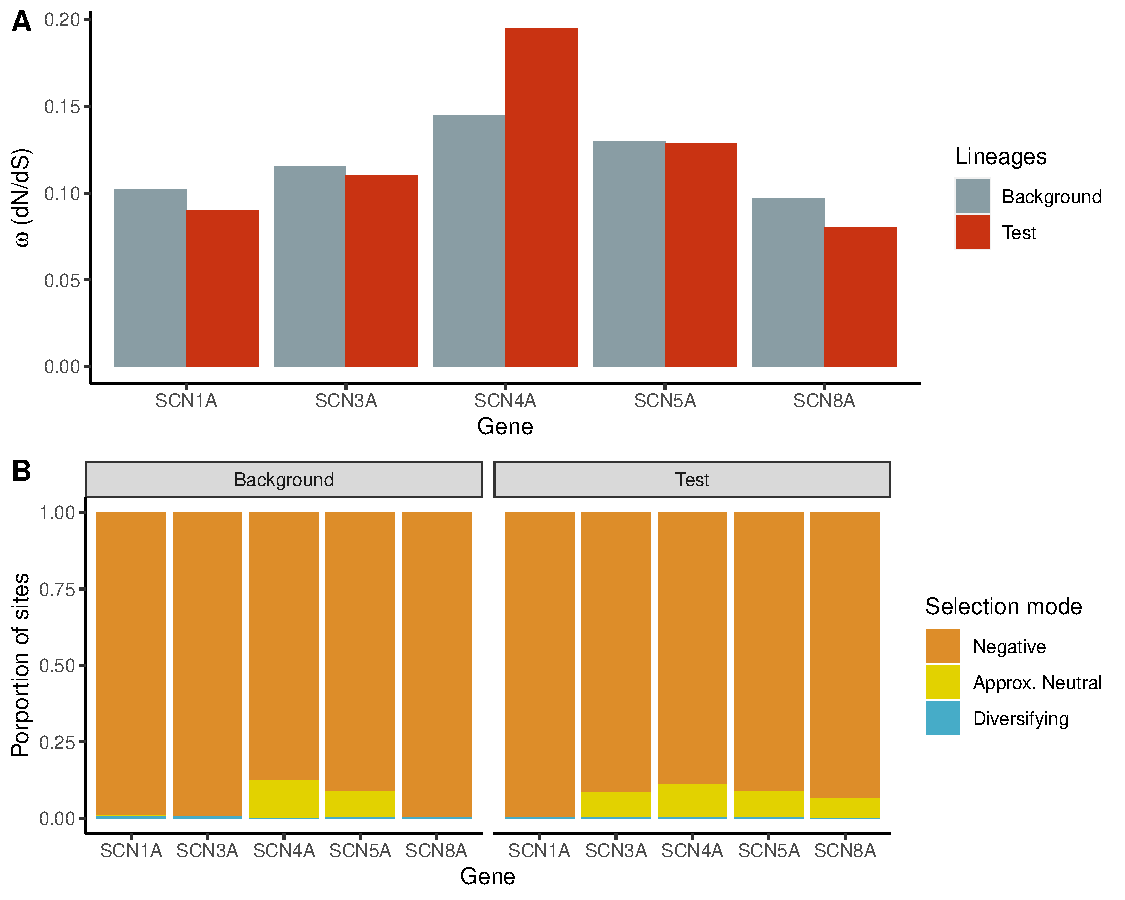
\includegraphics[width=\textwidth]{figures/Fig2_selection.pdf}
    \caption{Proportion of sites in each sodium channel gene that are negatively selected, neutral, or undergoing diversifying selection, as inferred by\texttt{BUSTED} as implemented in \texttt{HyPhy}. The left side of the plot (Background) corresponds to lineages that are known to be non-toxic or unknown toxicity, while the lineages in the Test group correspond to known toxic species and branches that are ancestral to clades of toxic species.}
    \label{fig:my_label}
\end{figure}
\clearpage

\begin{figure}[h!]
    \centering
    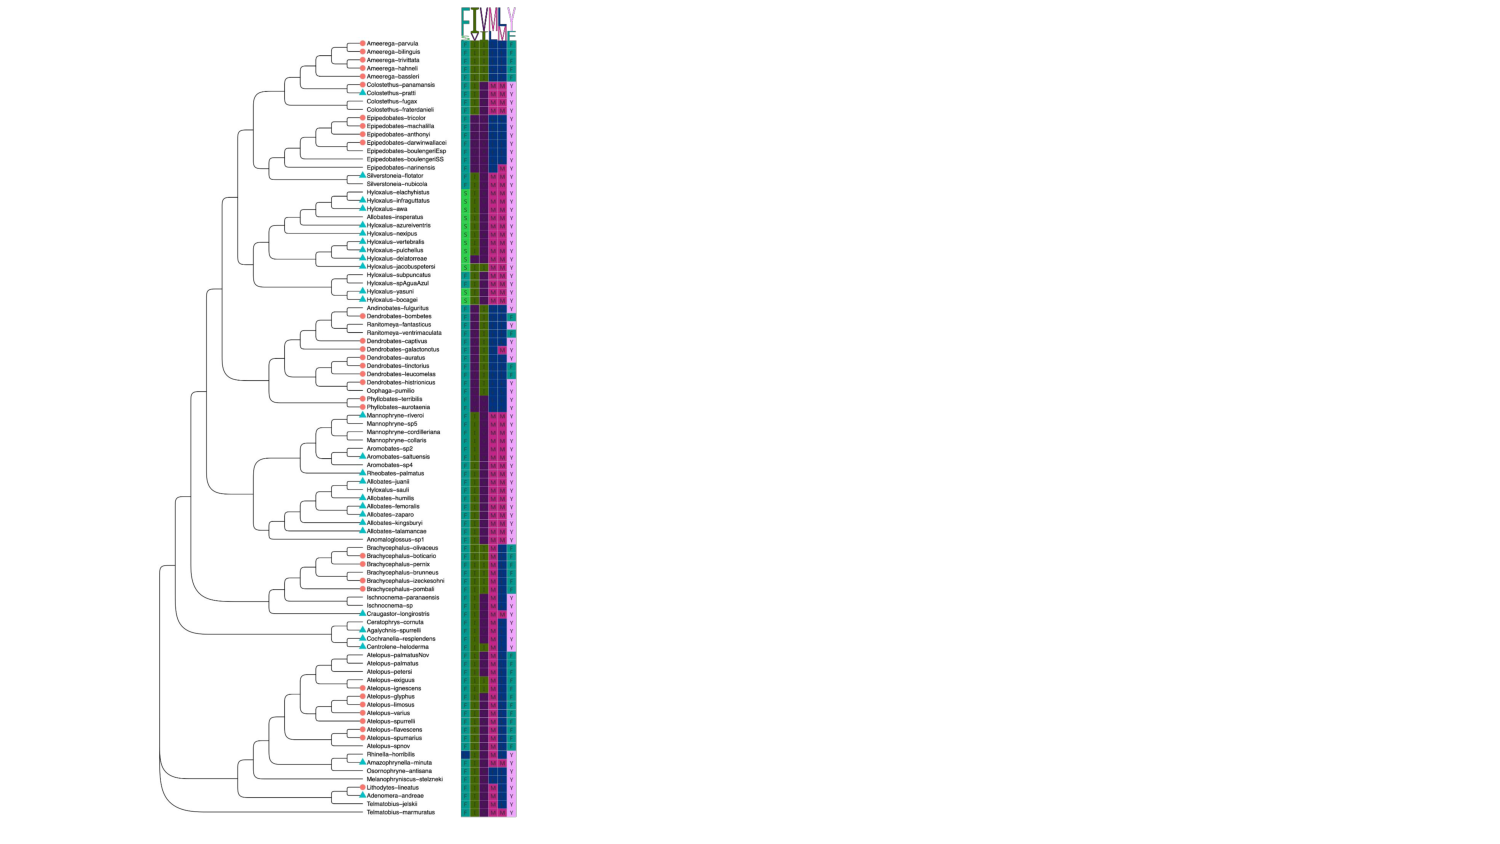
\includegraphics[width=0.6\textwidth]{figures/SCN4A.corrTree.trimmed.pdf}
    \caption{Gene tree of SCN4A plotted along with an alignment of six sites that are correlated with toxicity. Toxic species have a salmon colored dot, while non-toxic species have green triangles. We have no data on toxicity for unmarked species. The positions of the five correlated sites are given in Table 1, along with information about selection tests and the correlation with toxicity.}
    \label{fig:my_label}
\end{figure}
\clearpage

\begin{figure}[h!]
    \centering
    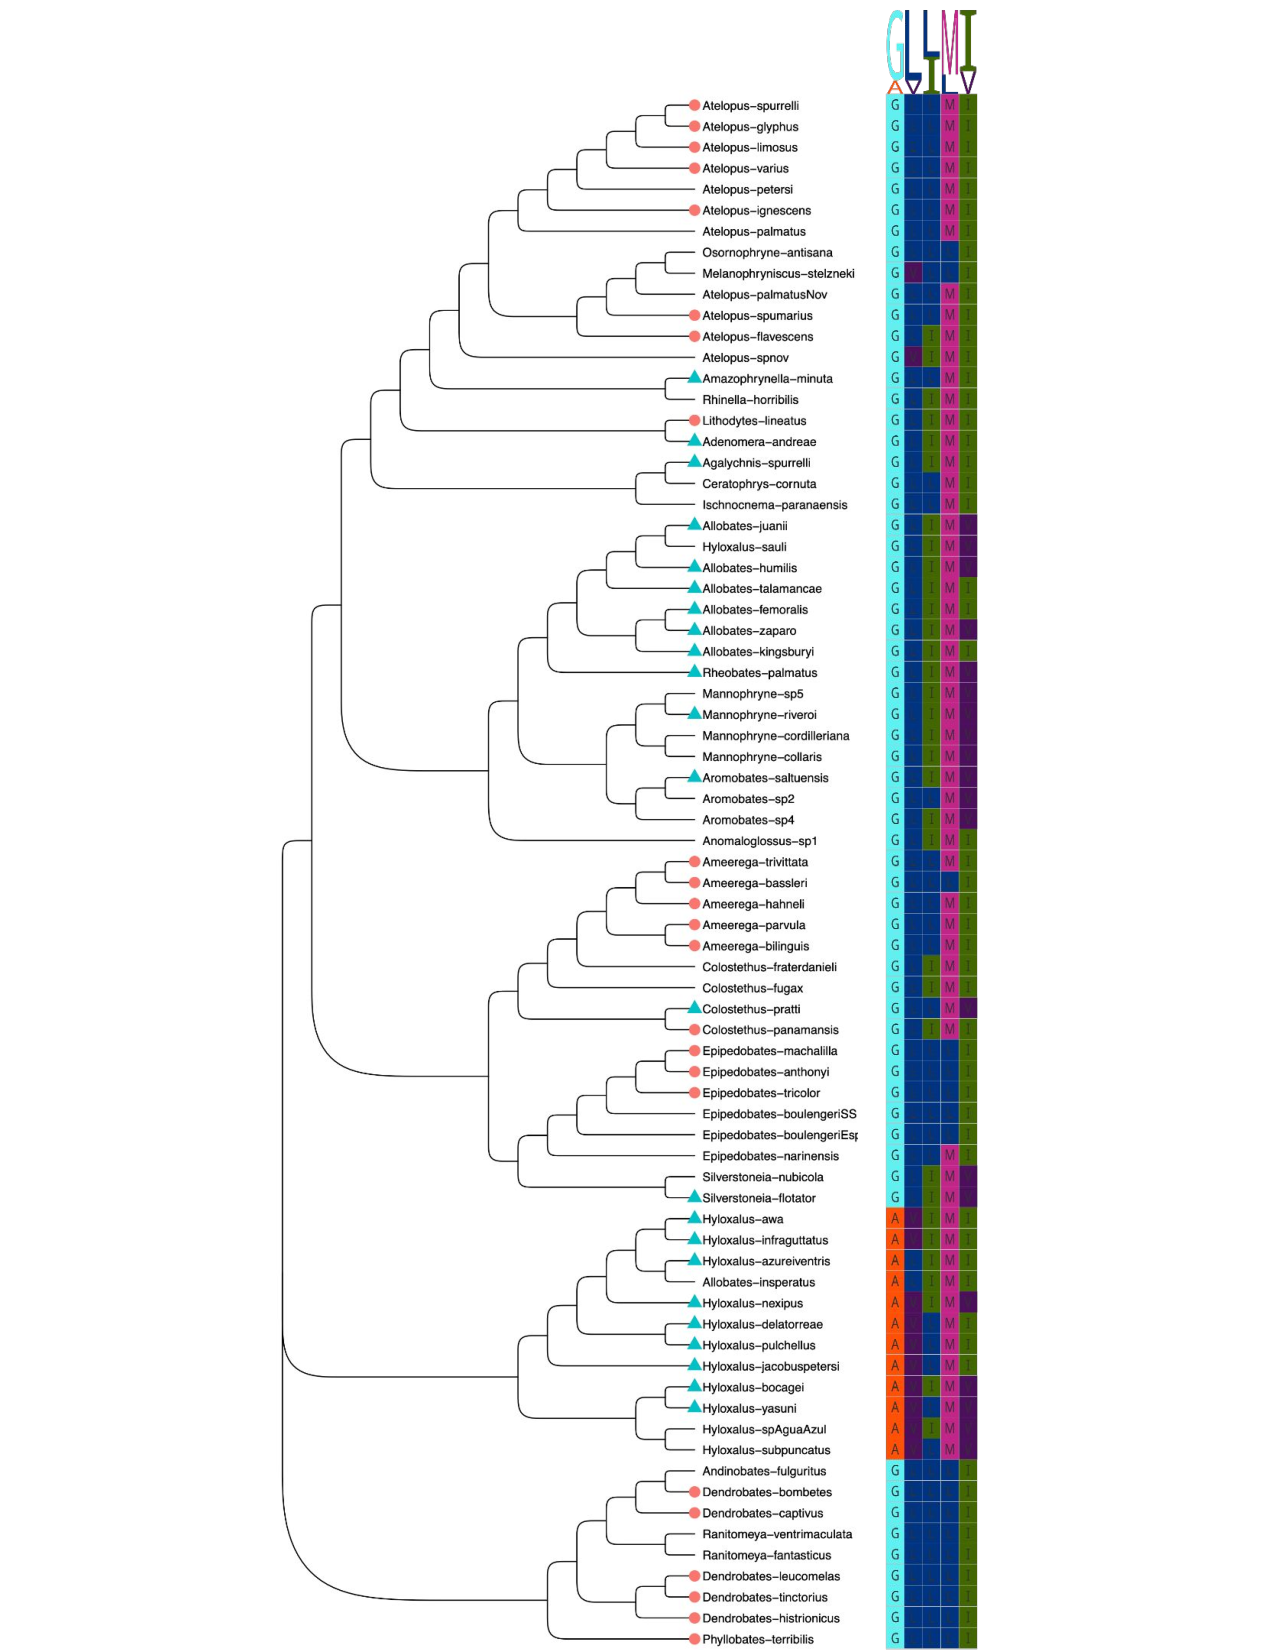
\includegraphics[width=0.85\textwidth]{figures/SCN5A.corrTree.trimmed.pdf}
    \caption{Gene tree of SCN5A plotted along with an alignment of five sites that are correlated with toxicity. Toxic species have a salmon colored dot, while non-toxic species have green triangles. We have no data on toxicity for unmarked species. The positions of the five correlated sites are given in Table 1, along with information about selection tests and the correlation with toxicity.}
    \label{fig:my_label}
\end{figure}
\clearpage

\begin{figure}[h!]
    \centering
    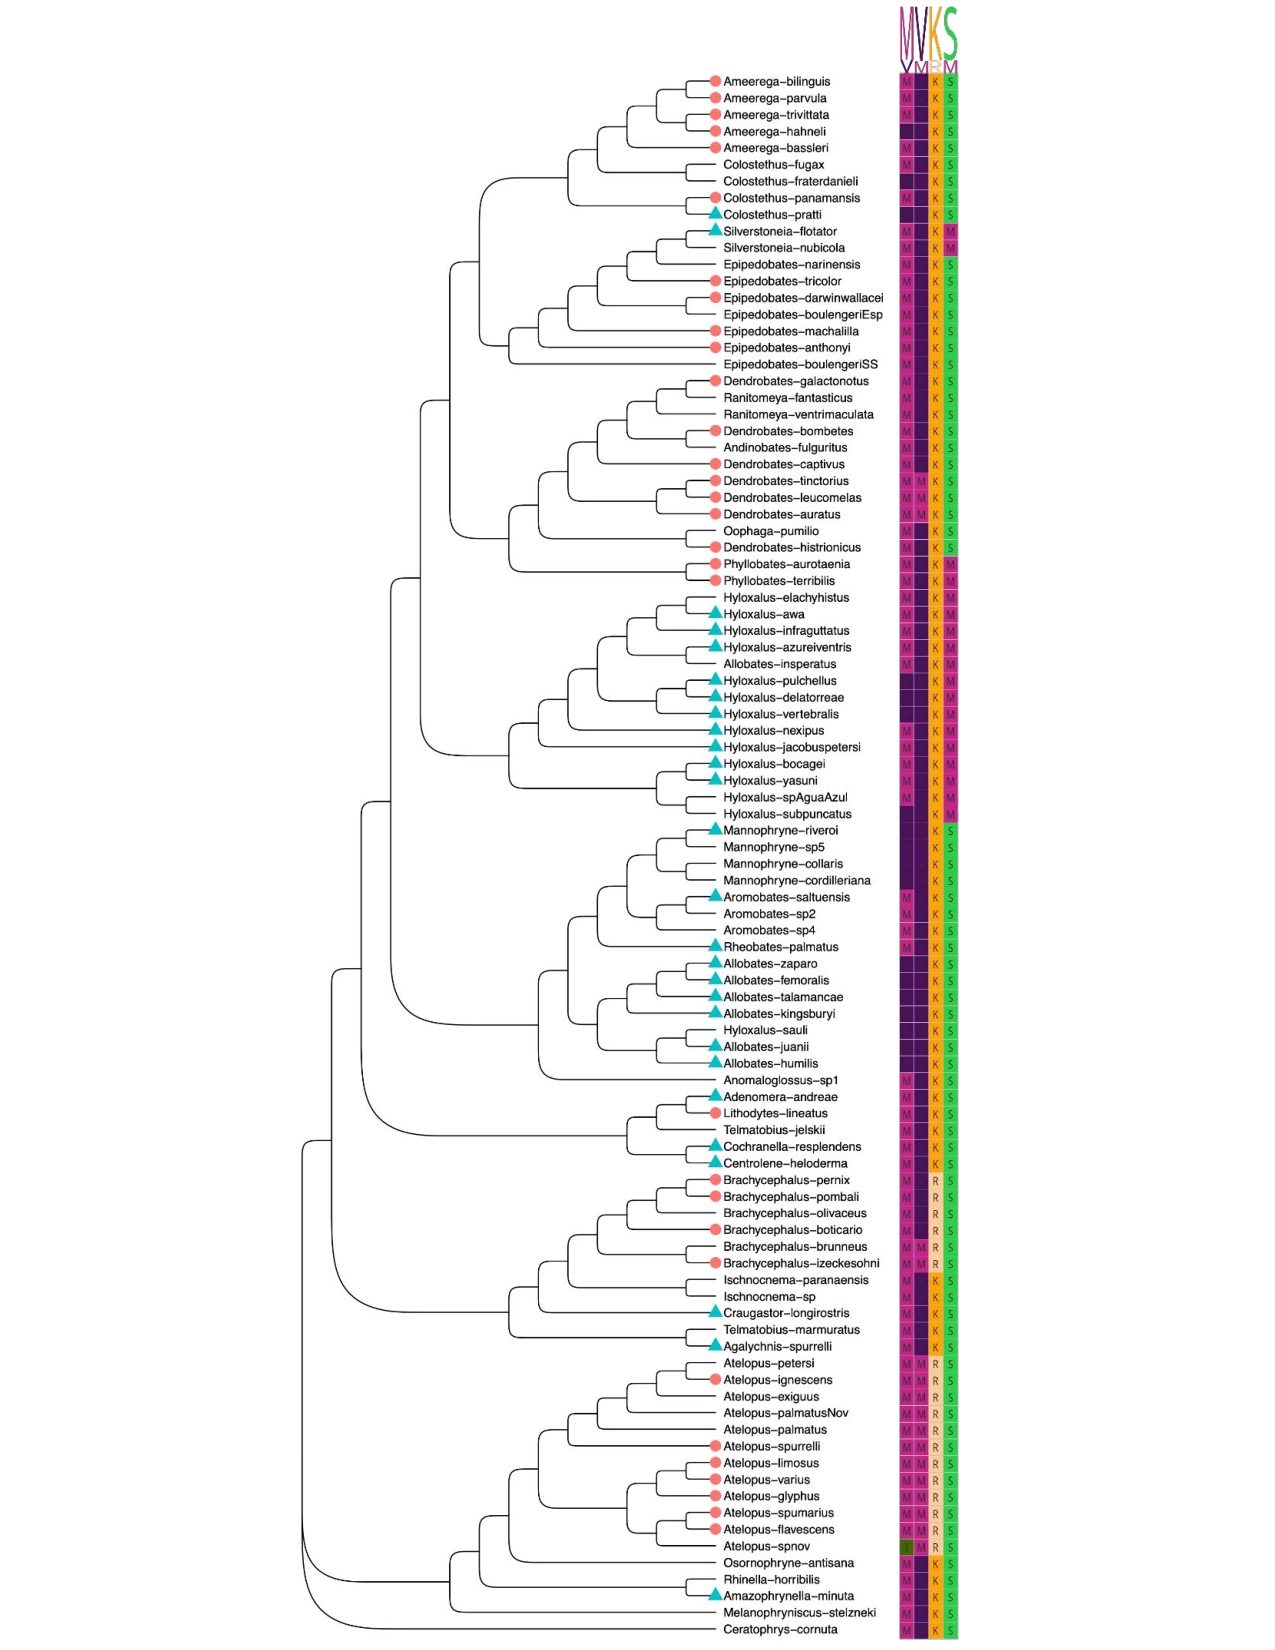
\includegraphics[width=0.85\textwidth]{figures/SCN8A.corrTree.trimmed.pdf}
    \caption{Gene tree of SCN8A plotted along with an alignment of four sites that are correlated with toxicity. Toxic species have a salmon colored dot, while non-toxic species have green triangles. We have no data on toxicity for unmarked species. The positions of the five correlated sites are given in Table 1, along with information about selection tests and the correlation with toxicity.}
    \label{fig:my_label}
\end{figure}
\clearpage

\begin{figure}[h!]
    \centering
    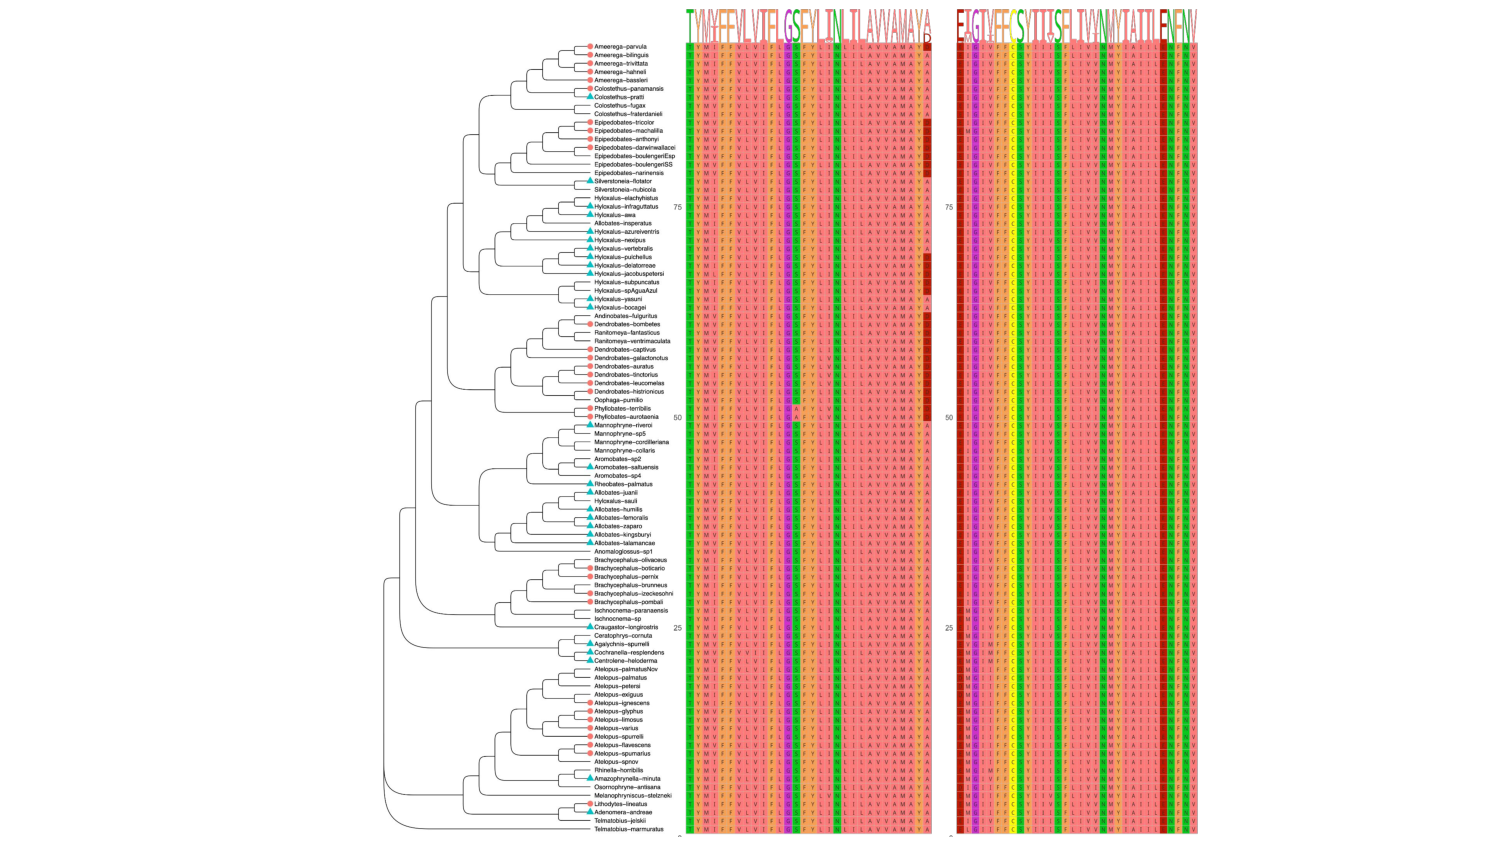
\includegraphics[width=\textwidth]{figures/Fig3_final.pdf}
    \caption{Multiple sequence alignment of sites near known toxicity resistance residues in SCN4A, along with the corresponding gene tree. Toxic species are marked with salmon colored dot, while non-toxic species have green triangles. The A $\rightarrow$D substitution at the end of the first block (position 445) of sites previously detected by \cite{tarvin2016convergent}.}
    \label{fig:my_label}
\end{figure}
\clearpage
\begin{table}
\centering
\begin{tabular}{ |p{3cm}||p{3cm}|p{3cm}|p{3cm}|p{3cm}|  }
 \hline
 \multicolumn{5}{|c|}{Sites correlated with toxicity} \\
 \hline
 Gene & Position & Substitution & PGLS p-value & MEME p-value \\
 \hline
       SCN3A & 1215 (1256) & N$\rightarrow$T & 3.88e-02  & 6.7e-01 \\
     SCN4A  & 301 (307) & F$\rightarrow$S & 4.15e-02 & 6.7e-01 \\
    SCN4A  & 638 (640) & V$\rightarrow$I & 1.22e-03 & 3.7e-01 \\
    SCN4A  & 748 (750) & V$\rightarrow$I & 2.45e-02 & 6.7e-01\\
    SCN4A &  777 (779) & M$\rightarrow$L & 1.13e-07 & 6.7e-01\\
    SCN4A & 1110 (1068) & M$\rightarrow$L & 1.46e-06 & 6.7e-01\\
     SCN4A & 1179 (1137) & Y$\rightarrow$F & 8.68e-04 & 8.1e-02$^{*}$\\
     SCN5A  & 69 (70) & G$\rightarrow$A & 4.44e-03 & 3.9e-01 \\
     SCN5A  & 96 (97) & L$\rightarrow$V & 3.93e-02 & 3.1e-02$^{**}$\\
     SCN5A  & 773 (489) & L$\rightarrow$I & 2.15e-02 & 4.5e-02$^{**}$ \\
    SCN5A & 777 (493) & L$\rightarrow$M & 8.03e-04 & 3.0e-01\\
    SCN5A & 1692 (1368) & I$\rightarrow$V & 9.38e-05 & 2.2e-01\\
    SCN8A & 649 (818) & M$\rightarrow$V & 4.71e-02 & 5.3e-01\\
    SCN8A & 921 (1086) & V$\rightarrow$M & 4.93e-02 & 5.6e-01\\ % poor alignment with reference
    SCN8A & 1502 (1591) & K$\rightarrow$R & 4.28e-03 & 6.7e-01\\
    SCN8A & 1573 (1661) & S$\rightarrow$M & 7.17e-03 & 1.9e-05$^{***}$\\
 \hline
\end{tabular}
\end{table}~\\~\\
\textbf{Table 1}: {Sites that were significantly correlated $(p<5e-2)$ with toxicity after performing a correction for phylogenetic structure. The first position in column 2 refer to the rat SCN4A sequence (accession AAA41682), while the position in parentheses refers to the column in our alignments. Sites that would have been identified as selected by \textit{MEME} are marked with an asterisk $(^*, p<0.1;\ ^{**}, p<0.05;\ ^{***}, p<1e-3)$}.
\clearpage

\bibliographystyle{plain}
\bibliography{mybib}

\clearpage

\setcounter{table}{0}
\renewcommand{\thetable}{S\arabic{table}}%
\setcounter{figure}{0}
\renewcommand{\thefigure}{S\arabic{figure}}%
\section*{Supplemental Figures }
\begin{figure}[h!]
    \centering
    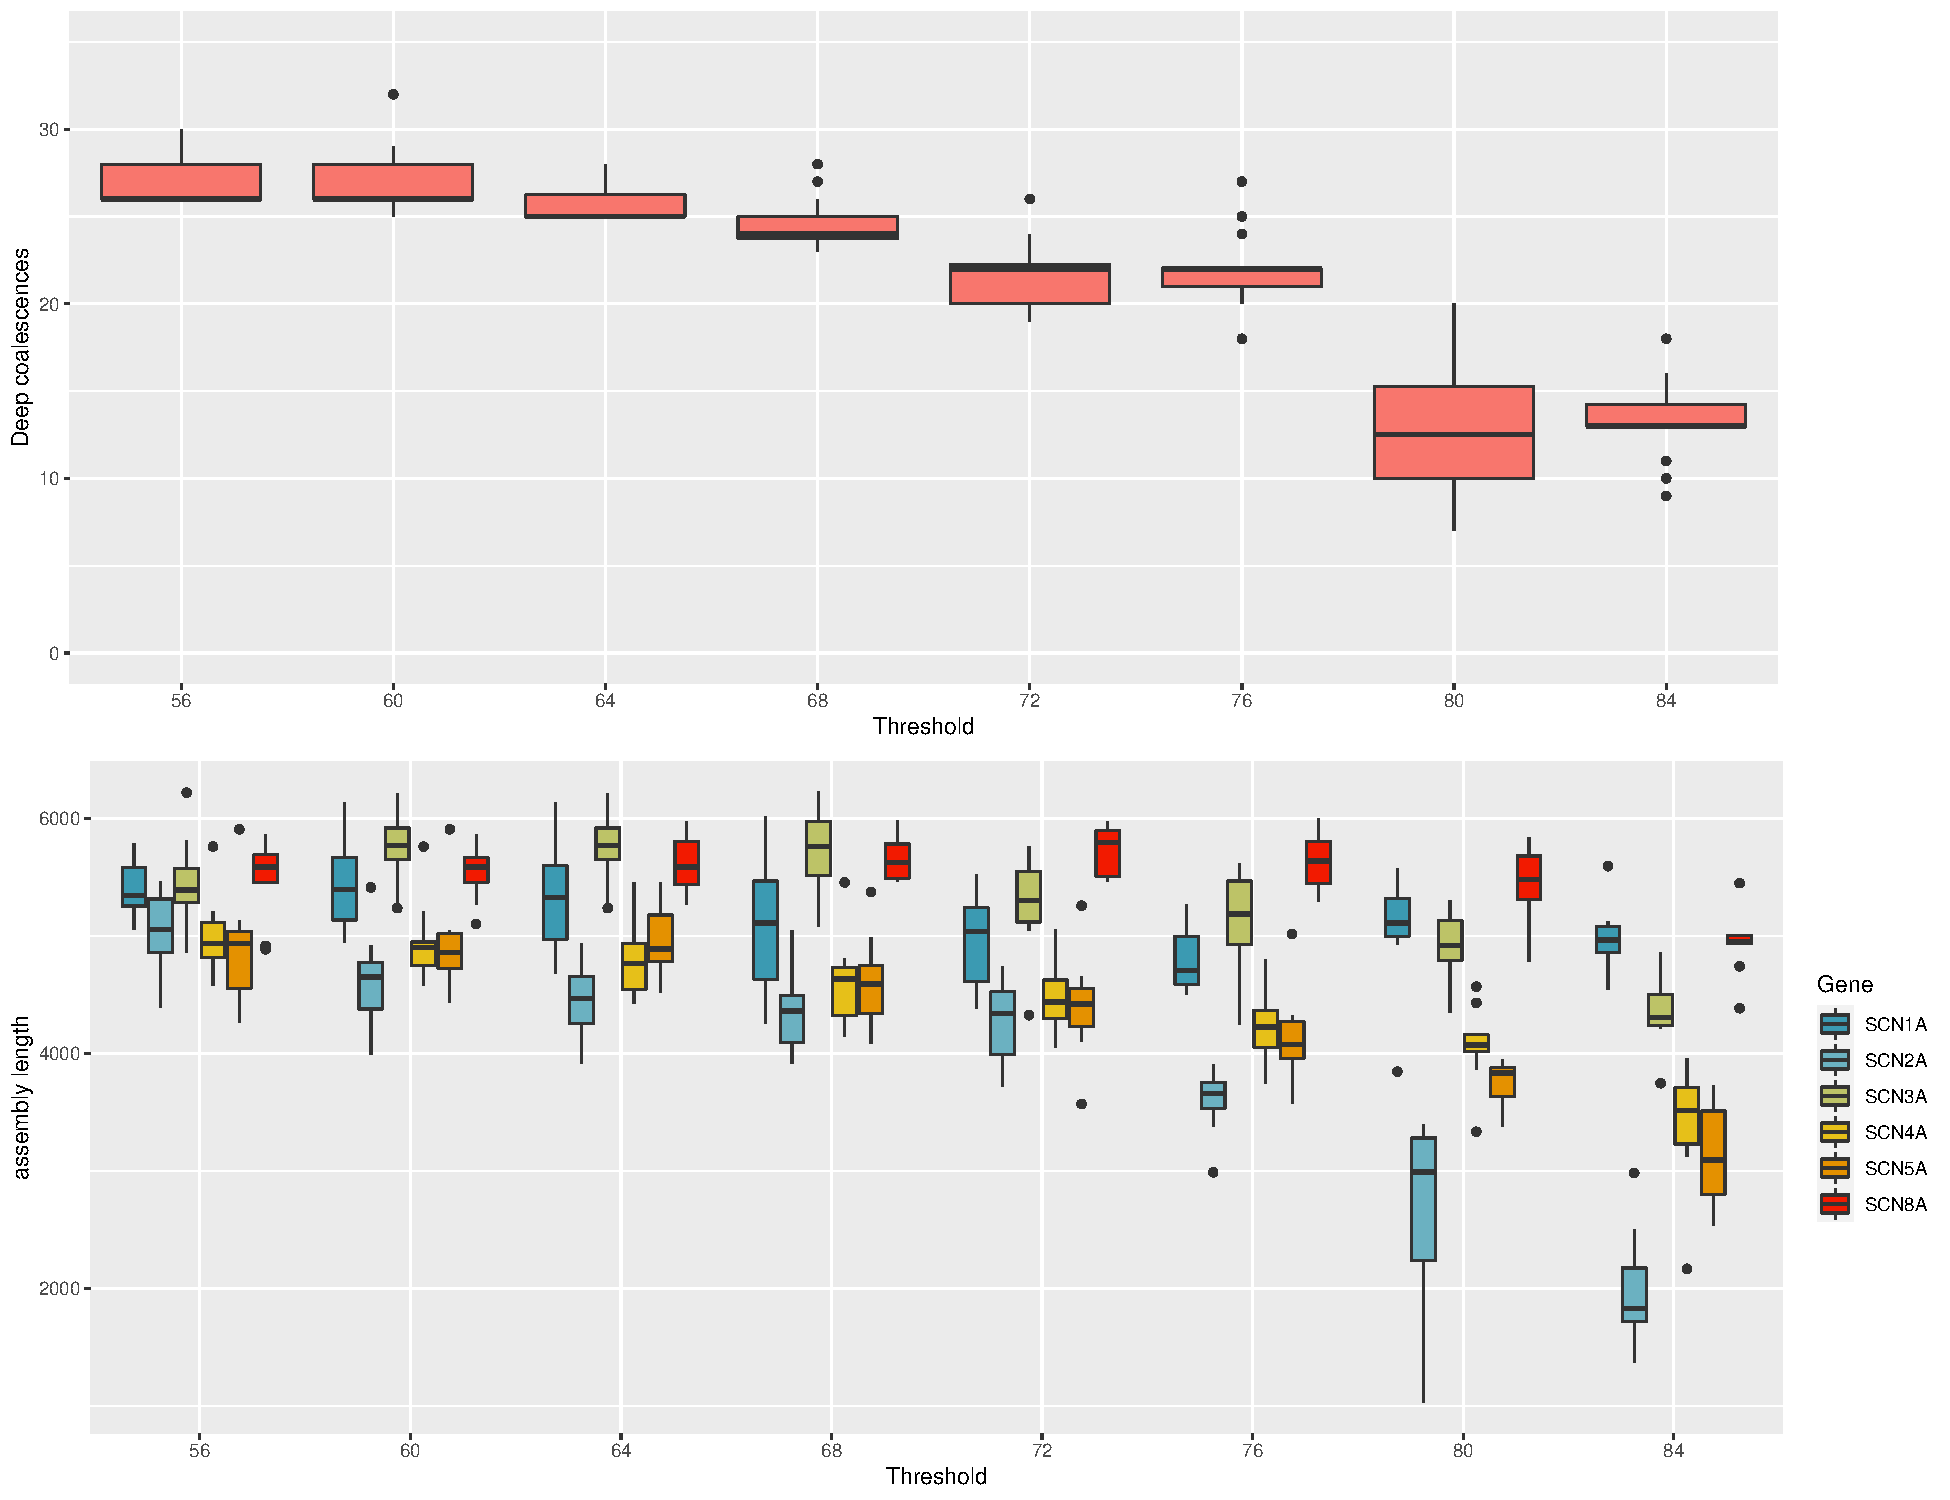
\includegraphics[scale=0.5]{figures/summary_alignments_xen_ref_orig.pdf}
    \caption{Summary of assemblies made with \textit{HybPiper} using a subset of frog species with \textit{Xenopus} bait sequences. The top panel shows the number of deep coalescences required to achieve reciprocal monophyly of all six sodium channel genes as a function of the percent-identity threshold for aligning contigs to the reference sequences parameter in \texttt{HybPiper}. The distributions correspond to 20 Maximum Likelihood trees obtained by \texttt{raxml-ng} for each assembly. The lower panel shows the length distribution of the assembled gene models for each gene as a function of the same threshold parameter.}
    \label{fig:my_label}
\end{figure}
\clearpage

\begin{figure}[h!]
    \centering
    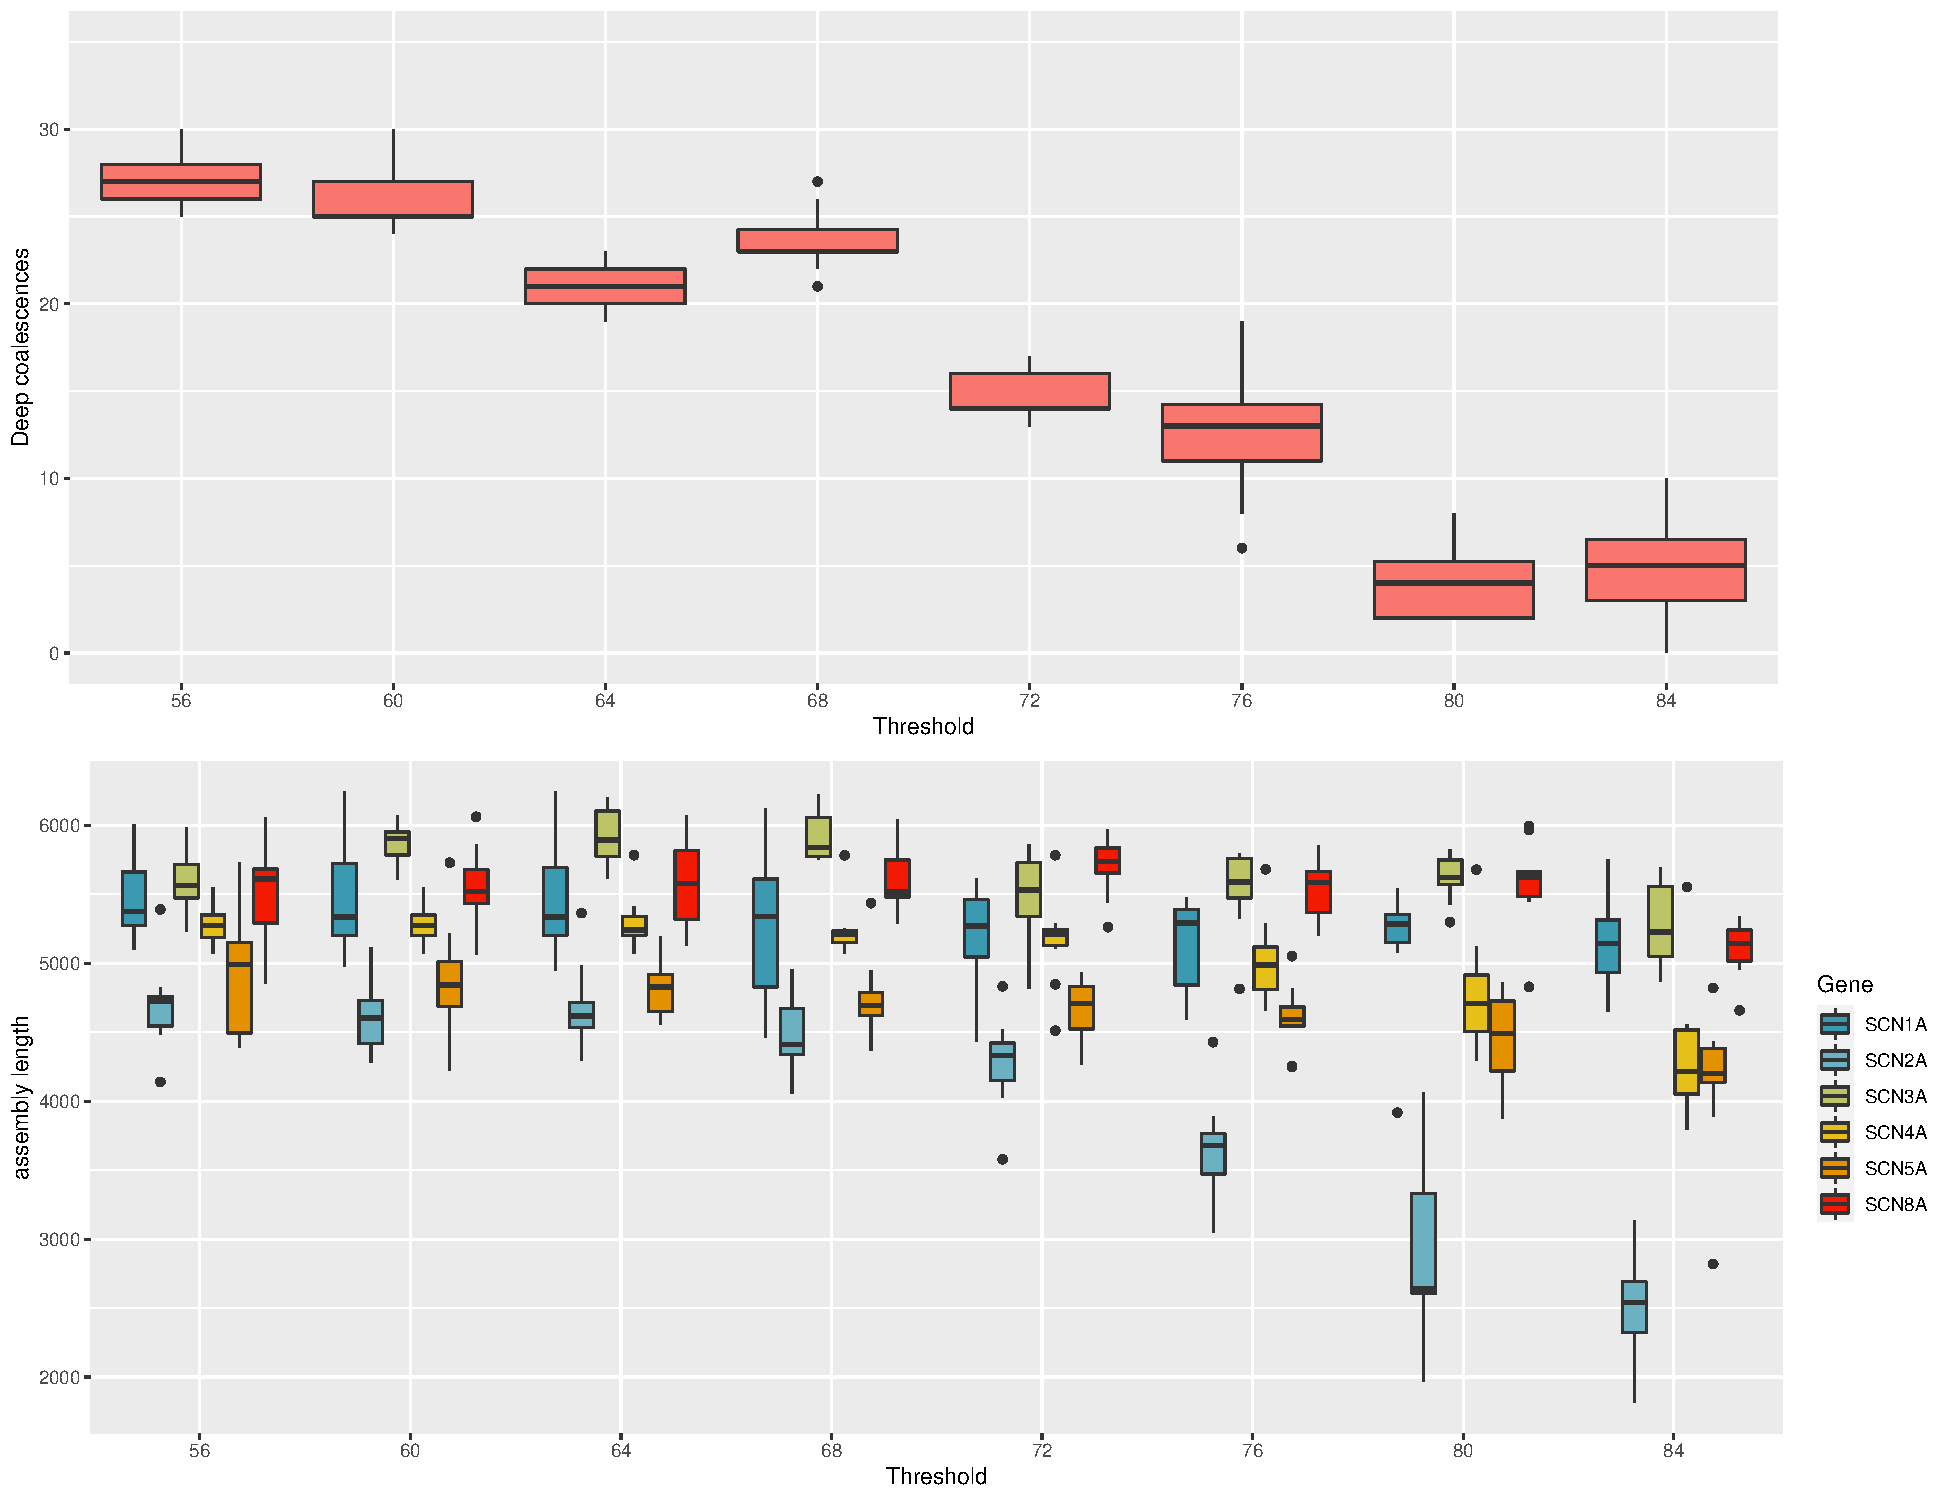
\includegraphics[scale=0.5]{figures/summary_alignments_xenPum_ref_orig.pdf}
    \caption{Summary of assemblies made with \texttt{HybPiper} using a subset of frog species with \textit{Xenopus}/\textit{Oophaga} hybrid bait sequences. The top panel shows the number of deep coalescences required to achieve reciprocal monophyly of all six sodium channel genes as a function of the percent-identity threshold for aligning contigs to the reference sequences parameter in \texttt{HybPiper}. The distributions correspond to 20 Maximum Likelihood trees obtained by \texttt{raxml-ng} for each assembly. The lower panel shows the length distribution of the assembled gene models for each gene as a function of the same threshold parameter.}
    \label{fig:my_label}
\end{figure}
\clearpage

\begin{figure}[h!]
    \centering
    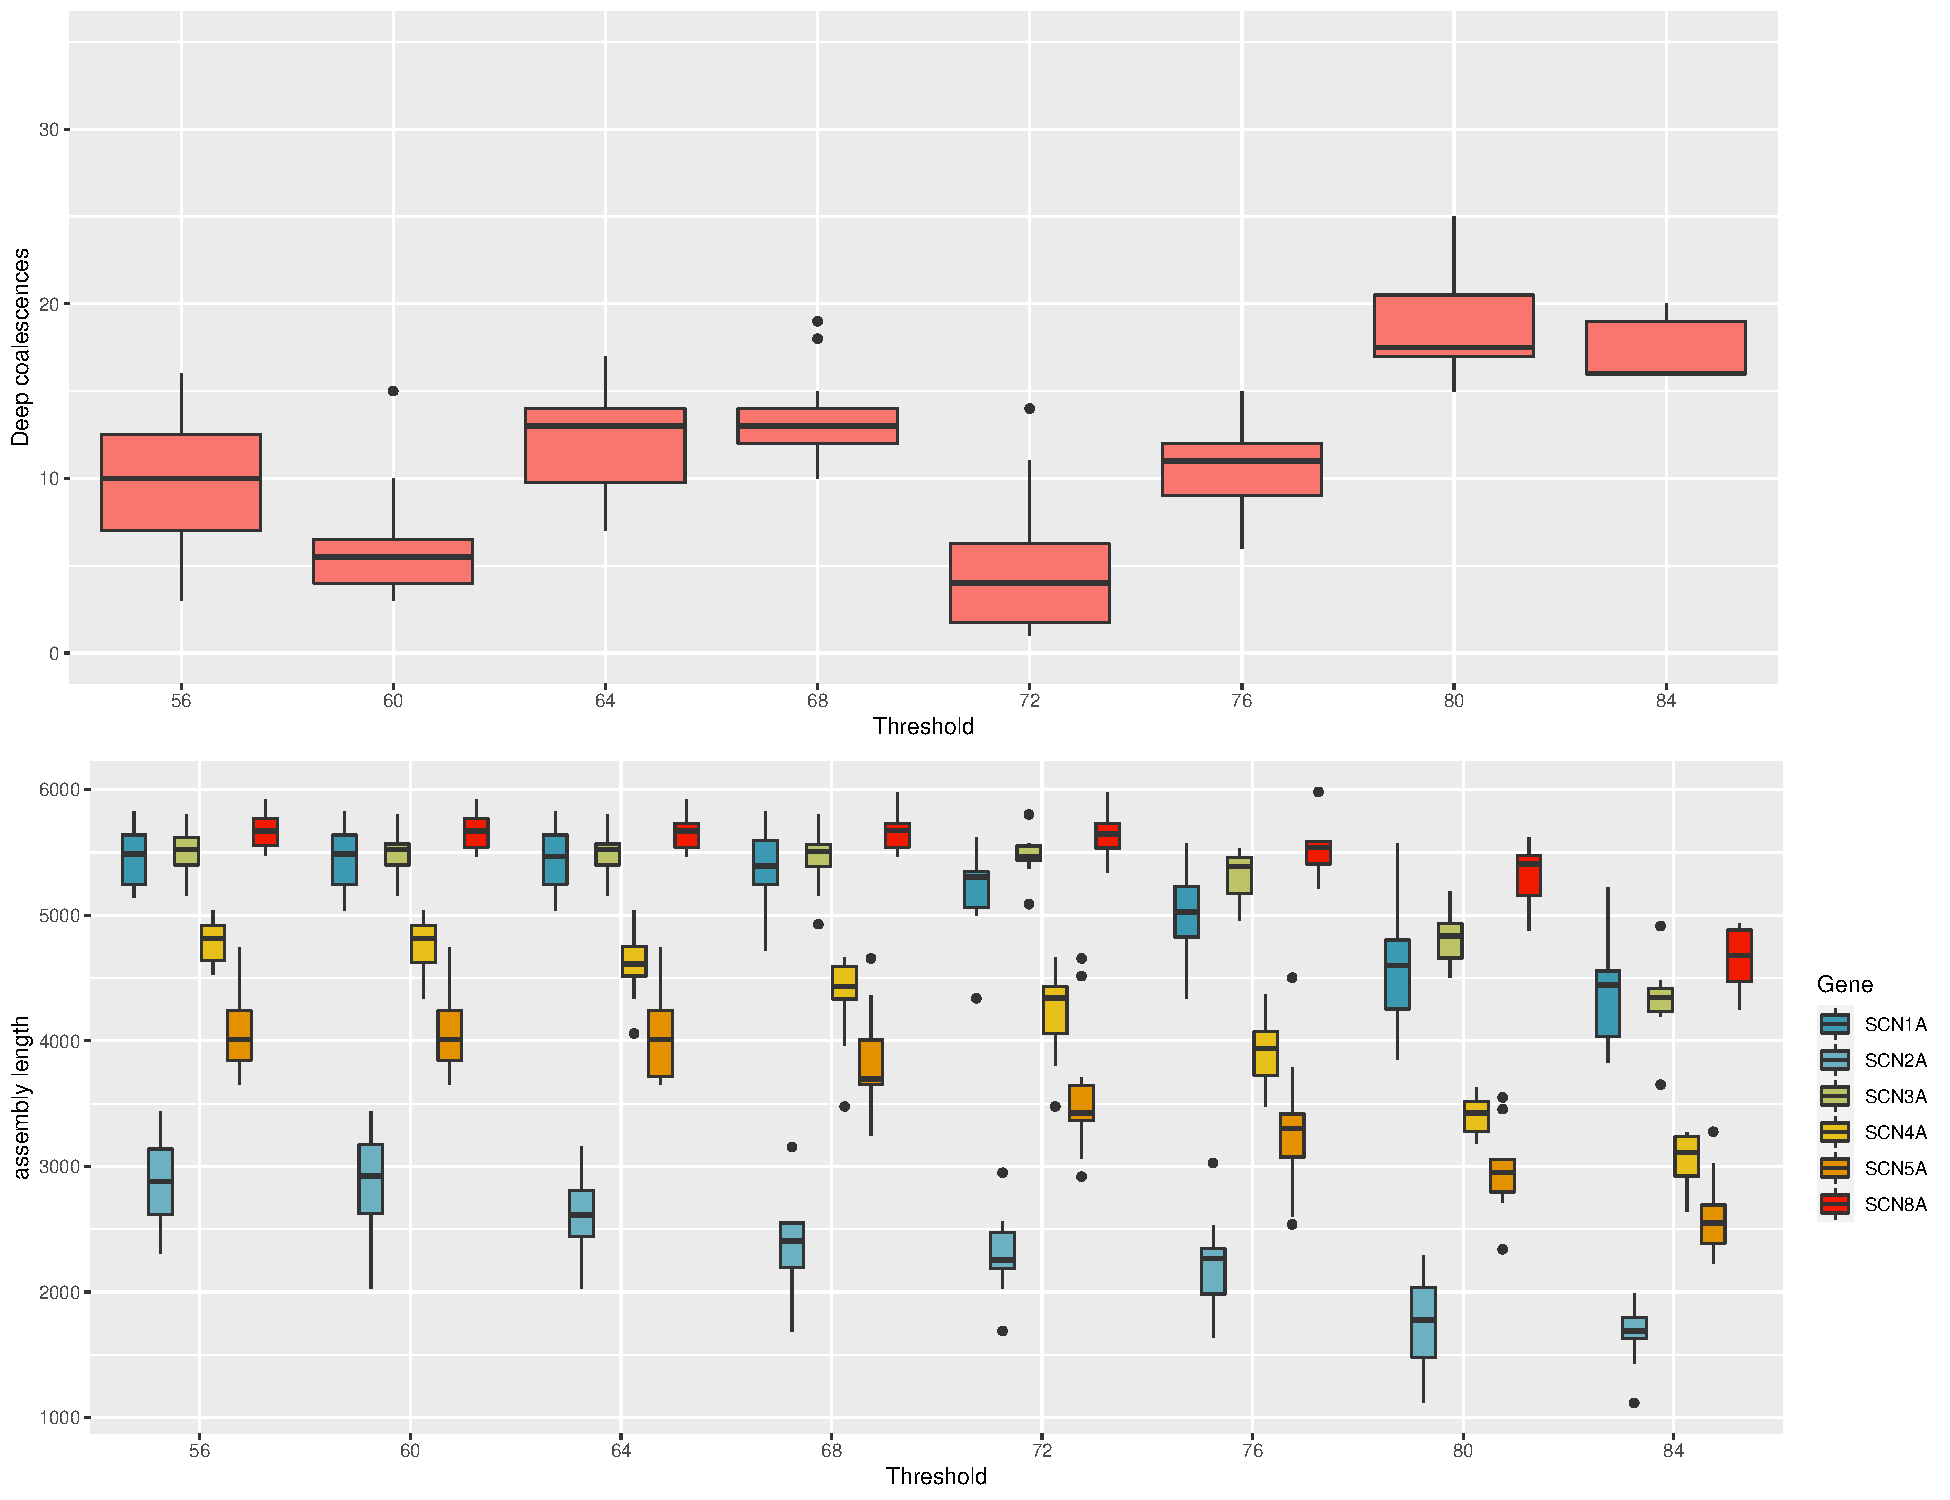
\includegraphics[scale=0.5]{figures/summary_alignments_xen_ref_HPfixed.pdf}
    \caption{Summary of assemblies made with a slightly modified version of \texttt{HybPiper} and a subset of frog species with \textit{Xenopus} bait sequences. The top panel shows the number of deep coalescences required to achieve reciprocal monophyly of all six sodium channel genes as a function of the percent-identity threshold for aligning contigs to the reference sequences parameter in \texttt{HybPiper}. The distributions correspond to 20 Maximum Likelihood trees obtained by \texttt{raxml-ng} for each assembly. The lower panel shows the length distribution of the assembled gene models for each gene as a function of the same threshold parameter.}
    \label{fig:my_label}
\end{figure}
\clearpage

\begin{figure}[h!]
    \centering
    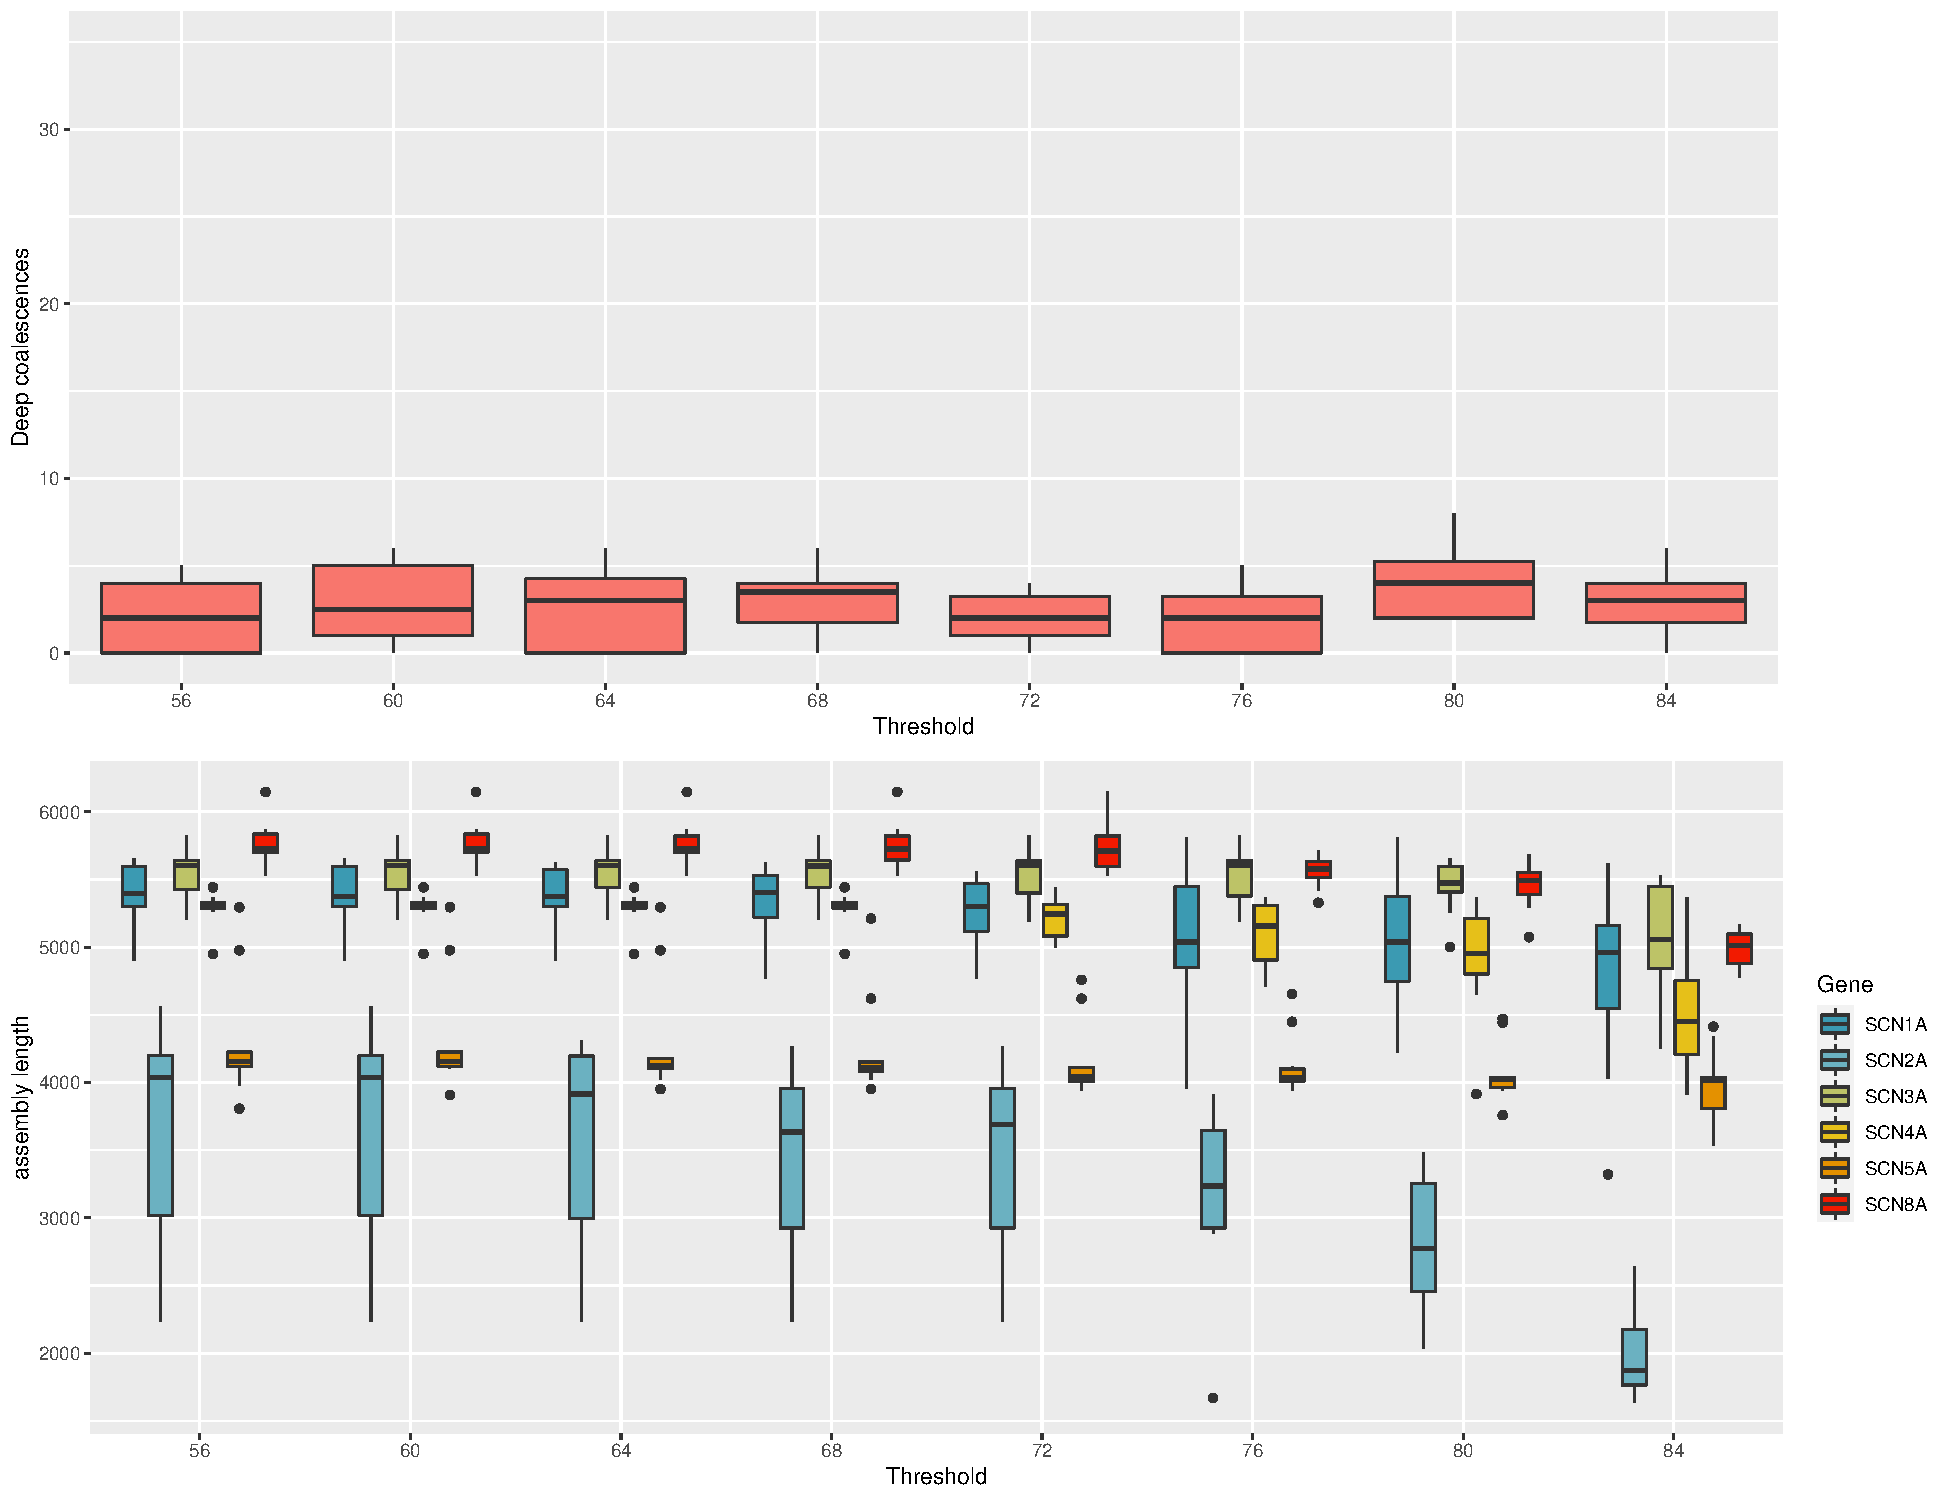
\includegraphics[scale=0.5]{figures/summary_alignments_xenPum_ref_HPfixed.pdf}
    \caption{Summary of assemblies made with a slightly modified version of \texttt{HybPiper} and a subset of frog species with \textit{Xenopus}/\textit{Oophaga} bait sequences. The top panel shows the number of deep coalescences required to achieve reciprocal monophyly of all six sodium channel genes as a function of the percent-identity threshold for aligning contigs to the reference sequences parameter in \texttt{HybPiper}. The distributions correspond to 20 Maximum Likelihood trees obtained by \texttt{raxml-ng} for each assembly. The lower panel shows the length distribution of the assembled gene models for each gene as a function of the same threshold parameter.}
    \label{fig:my_label}
\end{figure}
\clearpage

\begin{figure}[h!]
    \centering
    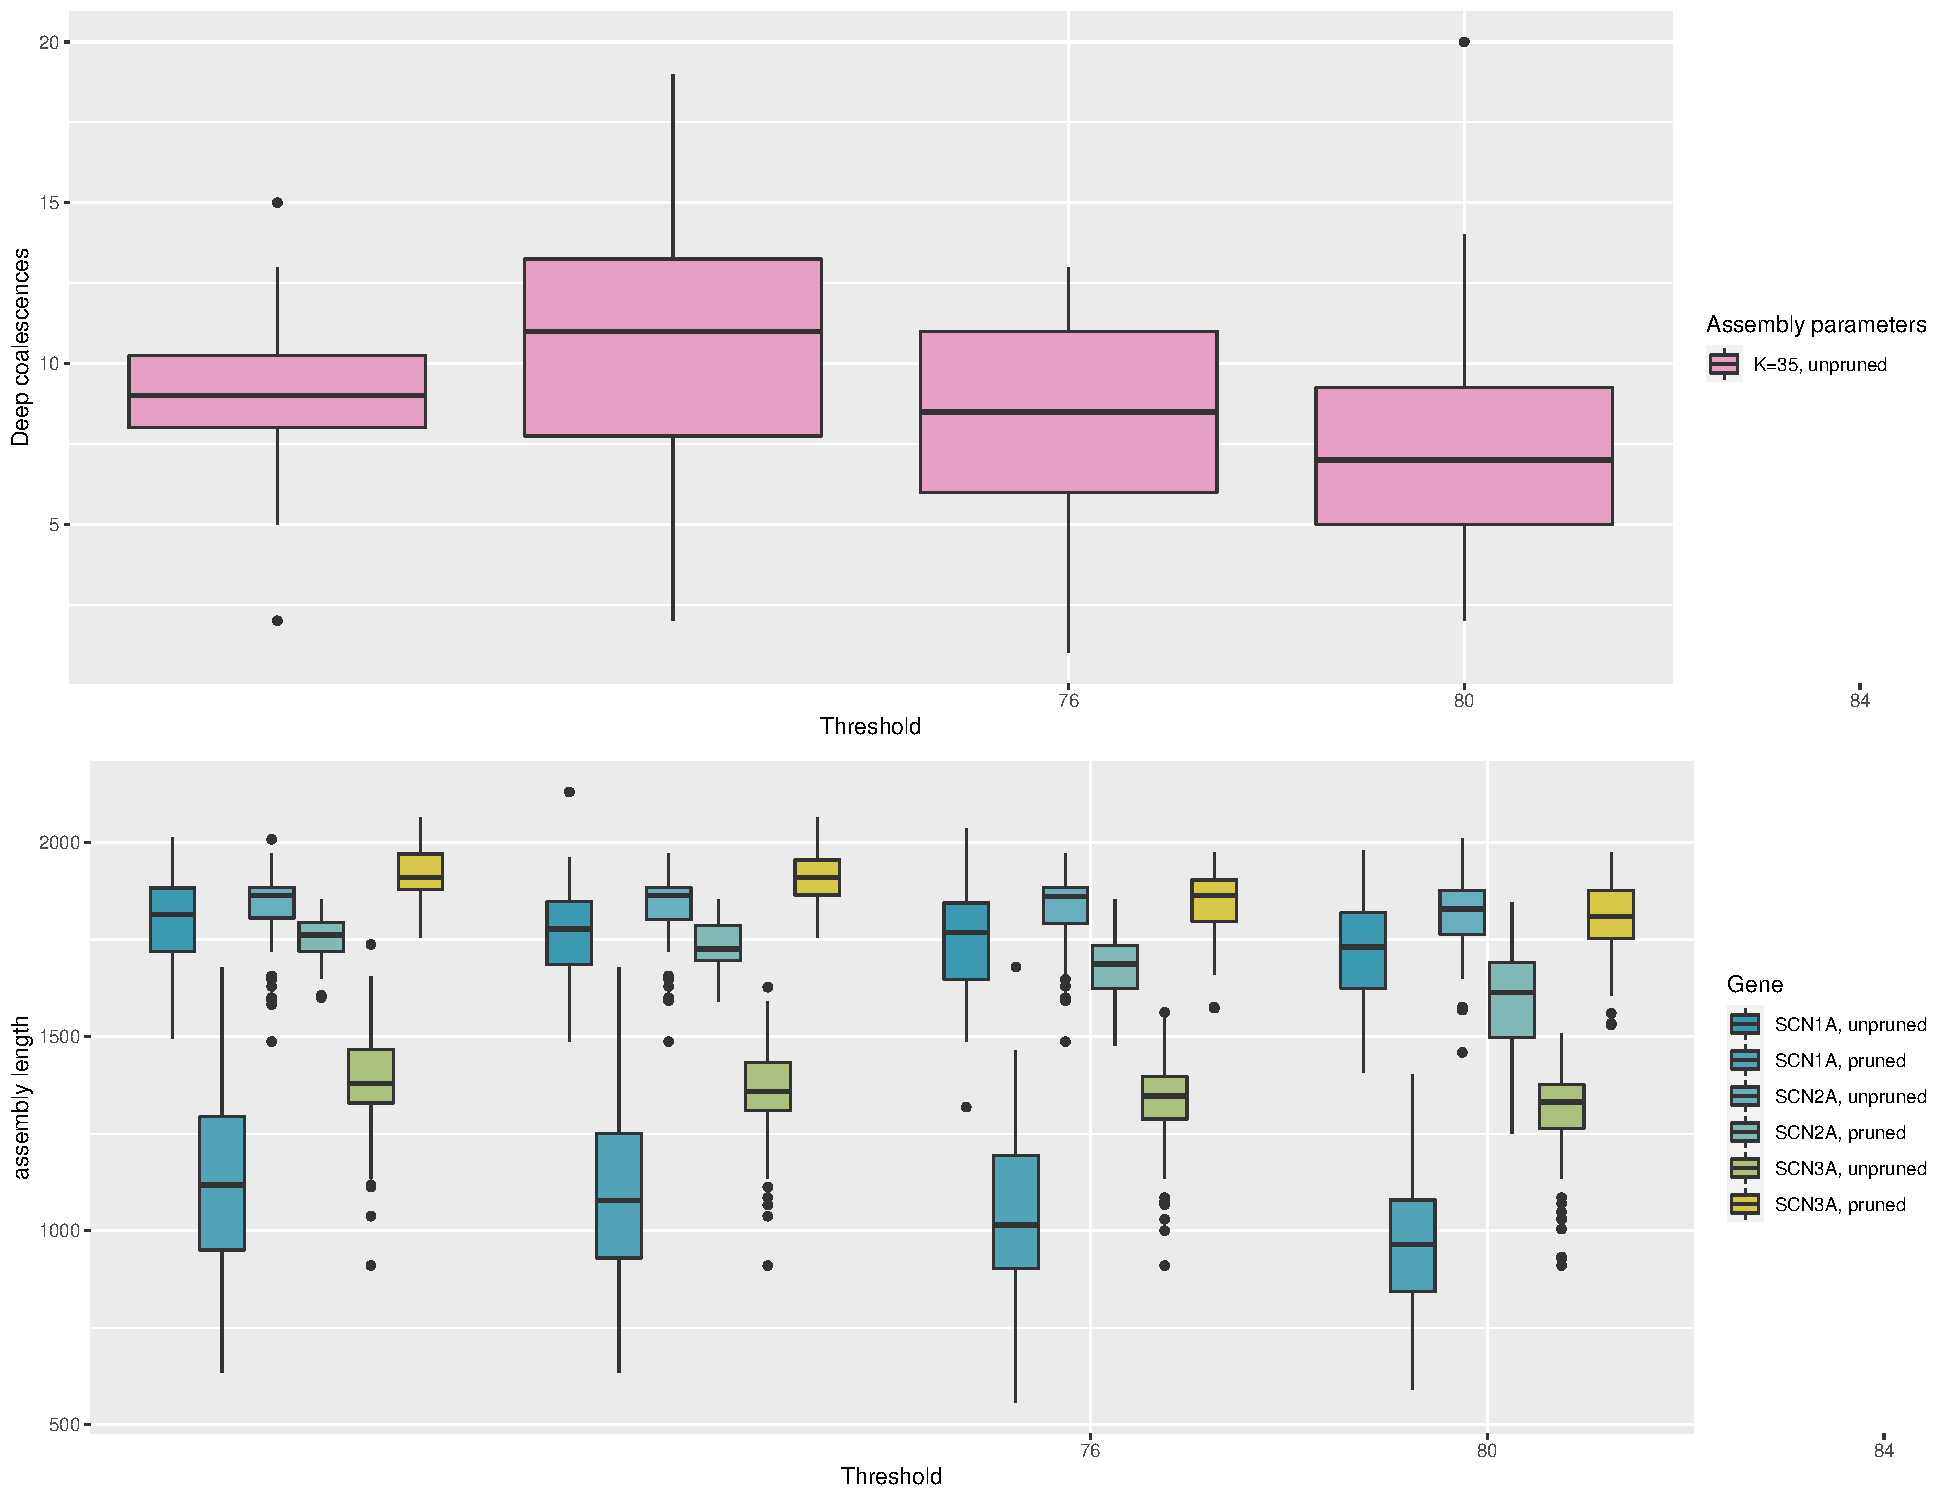
\includegraphics[scale=0.5]{figures/summary_alignments.pdf}
    \caption{Summary of assemblies made with a slightly modified version of \texttt{HybPiper} and all 95 frog species with \textit{Xenopus}/\textit{Oophaga} bait sequences. The top panel shows the number of deep coalescences required to achieve reciprocal monophyly of all six sodium channel genes as a function of the percent-identity threshold for aligning contigs to the reference sequences parameter in \texttt{HybPiper}. The lower panel shows the length distribution of the assembled gene models for each gene as a function of the same threshold parameter.}
    \label{fig:my_label}
\end{figure}
\clearpage

\begin{figure}[h!]
    \centering
    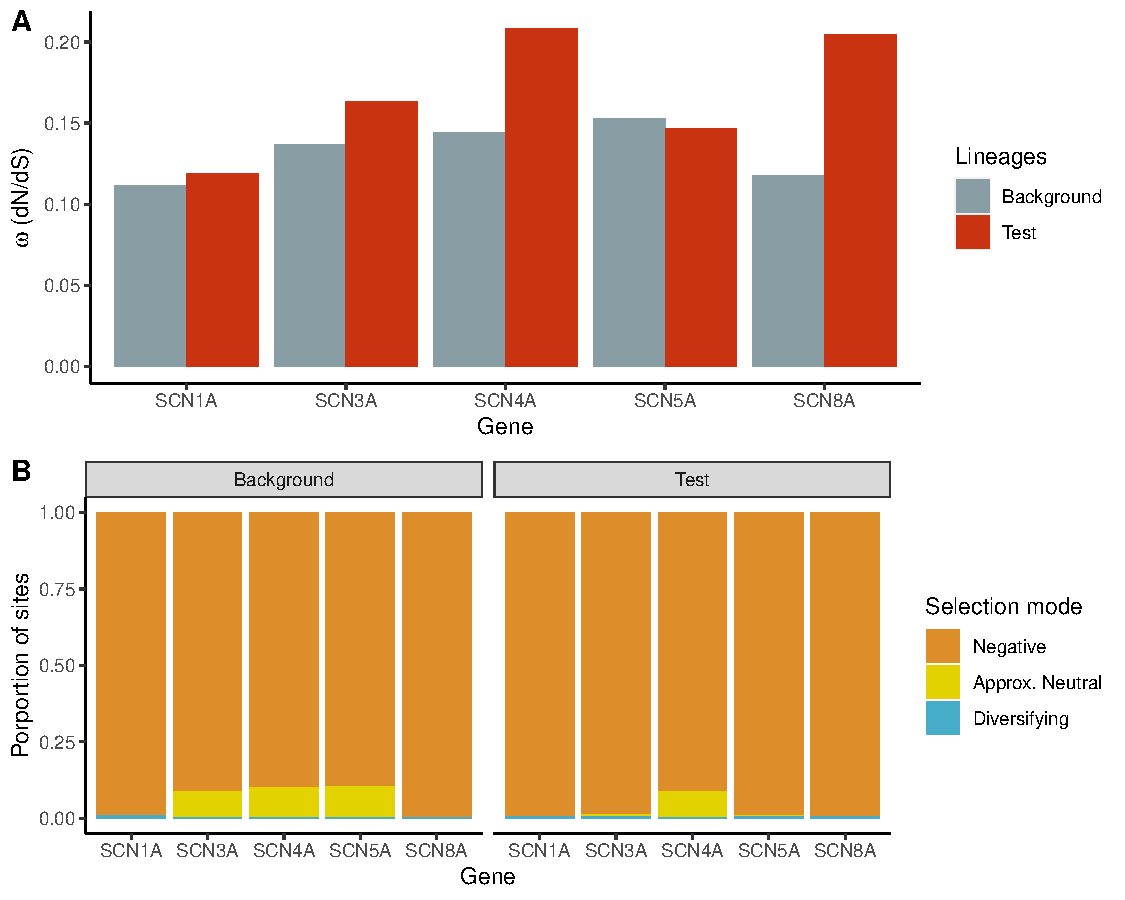
\includegraphics[width=\textwidth]{figures/FigS6_selection.pdf}
    \caption{Proportion of sites in each sodium channel gene that are negatively selected, neutral, or undergoing diversifying selection, as inferred by\texttt{BUSTED} as implemented in \texttt{HyPhy} and. a more conservative column-trimming strategy than in Fig.~2. The left side of the plot (Background) corresponds to lineages that are known to be non-toxic or unknown toxicity, while the lineages in the Test group correspond to known toxic species and branches that are ancestral to clades of toxic species.}
    \label{fig:my_label}
\end{figure}
\clearpage

%\tikzstyle{decision} = [diamond, draw, fill=blue!20, 
%    text width=4.5em, text badly centered, node distance=3cm, inner sep=0pt]
%\tikzstyle{block} = [rectangle, draw, fill=blue!20, 
%    text width=10em, text centered, rounded corners, minimum height=4em]
%    \tikzstyle{block} = [rectangle, draw, fill=blue!20, 
%    text width=10em, text centered, rounded corners, minimum height=12em]
%\tikzstyle{line} = [draw, -latex']
%\tikzstyle{cloud} = [draw, ellipse,fill=red!20, node distance=3cm,

%\begin{tikzpicture}[node distance = 2cm, auto]
    % Place nodes
 %   \node [block] (init) {Trim adapters and low quality sequences};
 %   \node [longblock, below of=init] (identify) {Run HybPiper};
 %   \node [block, below of=identify] (evaluate) {evaluate candidate models};

 %   \node [decision, below of=evaluate] (decide) {is best candidate better?};
 %   \node [block, below of=decide, node distance=3cm] (stop) {stop};
    % Draw edges

 %   \path [line] (decide) -| node [near start] {yes} (update);
 %   \path [line] (update) |- (identify);

%\end{tikzpicture}



\end{document}
